Farbladung hat drei m\"ogliche Zust\"ande: rot, blau und gr\"un.
Dabei spielt der Zustand der Farbladung f\"ur die St\"arke der starken Wechselwirkung keine Rolle.
Zus\"atzlich zu den drei Zust\"anden der Farbladung gibt es auch drei Zust\"ande der Antifarbladung. 
Die drei Zust\"ande der Antifarbladung sind entsprechend antirot, antiblau und antigr\"un.
Die Kombination der drei (Anti-)Farbladungen, oder die Kombination Farbladung mit passender Antifarbladung ergibt, angelehnt an die Farblehre, die Farbladung wei{\ss}.
Die Farbladung enth\"alt keine Information \"uber die tats\"achliche Farbe der Teilchen.
Teilchen mit dem wei{\ss}en Zustand als Farbladung entsprechen nach au{\ss}en hin farbneutralen Teilchen, auch wenn sie aus farbgeladenen Teilchen aufgebaut sind.
\newline
Quarks, Antiquarks und Gluonen tragen jeweils Farbladung, wodurch sie an der starken Wechselwirkung teilnehmen.
Unter anderem bindet die starke Wechselwirkung Quarks und Antiquarks zu sogenannten Hadronen. %Ungenau formuliert, weil qqbar ist Meson, wir wollen allgemein
Hadronen werden wiederum in sogenannte Baryonen, aufgebaut aus drei Quarks, und sogenannte Mesonen, aufgebaut aus einem Quark-Antiquark Paar und entsprechende Antiteilchen unterteilt.
In der Natur kommen nur farbneutrale Teilchen vor, es gibt keine freie Farbladung.
Entsprechend gibt es (Anti-)Quarks nur in Zusammenschl\"ussen und nicht frei. 
Dieses Ph\"anomen wird als \textit{Confinement} bezeichnet.
Um das \textit{Confinement} besser verstehen zu k\"onnen wird im Folgenden das Potential der starken Wechselwirkung erl\"autert.
\newline
%AKTUELLER STAND%%%%%%%%%%%%%%%%%%%%%%%%%%%%%%%%%%%%%%%%%%%%%%%%%%%%%%%%%%%%
Die Kraft, die auf farbgeladene Teilchen wirkt, folgt aus einem Potential $V(r)$.
Dieses $V(r)$ besitzt einen anziehenden Teil und einen abstoßenden Teil.
Der anziehende Teil weist dabei eine Proportionalit\"at zum Abstand $r$ zweier farbgeladener Teilchen auf, w\"ahrend der absto{\ss}ende Teil eine Antiproportionalit\"at zu $r$ aufweist.
Der absto{\ss}ende Teil ist zus\"atzlich proportional zur sogenannten Kopplungskonstante der starken Wechselwirkung $\alpha_\text{s}$.
Es gilt:
\begin{align} \label{eq:Potential}
V(r) = -\frac{4}{3}\frac{\alpha_\text{s}}{r} + kr 
\end{align}
F\"ur gro{\ss}e $r$ wird der anziehende Teil also immer stärker.
Will man also zwei farbgeladene Teilchen wie etwa ein Quark-Antiquark-Paar von einander trennen, so m\"usste man immer mehr Energie aufwenden, je weiter man die Teilchen von einander entfernt.
Ab einem bestimmten Punkt wird die ben\"otigte Energie so gro{\ss}, dass sie ausreicht ein weiters Quark-Antiquark-Paar zu erzeugen.
Diese Erzeugung eines neue Quark-Antiquark-Paares findet immer statt sobald sie m\"oglich ist.
Deshalb sind Quarks und Gluonen nicht direkt einzeln messbar, was die Untersuchung von Quarks, Gluonen und der starken Wechselwirkung erschwert.
Um zu erkl\"aren, wie die starke Wechselwirkung, Quarks und Gluonen trotzdem untersuchen werden k\"onnen muss man sich $\alpha_\text{s}$ genauer anschauen. 
\newline
\begin{figure}[thp]
\centering
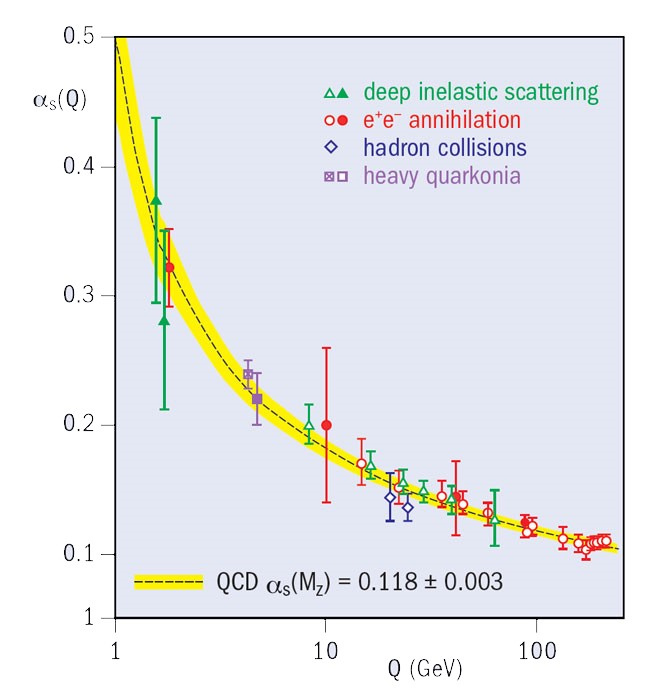
\includegraphics[width=.5\linewidth]{alpha_s.jpg}
\caption{Die Kopplungskonstante der starken Wechselwirkung $\alpha_\text{s}$ in Abh\"angigkeit des Impulsübertrags $Q$. Eingezeichnet befinden sich Messpunkte unterschiedlicher Experimente, sowie in gelb eine theoretische Rechnung.
\cite{article:1}}
\label{fig:alpha_2}
\end{figure}
Anders als die Bezeichnung vermuten l\"asst ist die Kopplungskonstante nicht konstant.
Stattdessen h\"angt $\alpha_\text{s}$ vom sogenannten Impulsübertrag $Q$ zwischen zwei Teilchen ab.
Abbildung \ref{fig:alpha_2} zeigt den Verlauf von $\alpha_\text{s}$ in Abh\"ahngigkeit von $Q$.
Der Impulsübertrag $Q$ h\"angt dabei selbst \"uber die De-Broglie-Wellenl\"ange mit dem Abstand $r$ zusammen.
Es gilt $Q = \frac{h}{\lambda}$, wobei $\lambda$ die r\"aumliche Aufl\"osung beschreibt.
F\"ur eine genau Aufl\"osung, also f\"ur  sehr kleine $r$ muss entsprechend $Q$ gro{\ss} sein.
$\alpha_\text{s}$ h\"angt also antiproportional von $r$ ab.
Aufgrund dieser Abh\"angigkeit von $\alpha_\text{s}$ bez\"uglich $Q$ beziehungsweise $r$ nennt man $\alpha_\text{s}$ auch \textit{running $\alpha_\text{s}$}. 
Den Zustand f\"ur sehr kleine $\alpha_\text{s}$ nennt man asymptotische Freiheit, da sich innerhalb dieses Zustands Quarks und Gluonen quasi frei bewegen k\"onnen.
Um so einen Zustand erzeugen zu k\"onnen braucht man eine hohe Dichte von Quarks und Gluonen oder eine hohe Temperatur.
Eine verbreitete theoretische Beschreibung eines Mediums in diesem hei{\ss}en und dichten Zustand ist das sogenannte Quark-Gluon-Plasma, kurz QGP.
\newline
Ein solcher hei{\ss}er und dichter Zustand entsteht kurz nach der Kollision von zwei hochenergetischen Atomkernen.
Quarks und Gluonen, die aus diesem Medium kommen, m\"ussen, w\"ahrend der sogenannten Hadronisierung, wieder zu Hadronen werden.
Diese Hadronen k\"onnen zerfallen, insofern sie keine stabilen Teilchen sind.
Es kann auch zu ganzen Zerfallsketten kommen, bis die Endteilchen nicht mehr zerfallen.
Je nach dem, wie schnell Teilchen zerfallen, k\"onnen entweder diese oder ihre Zerfallsprodukte gemessen werden und liefern indirekt Aufschluss auf Eigenschaften des hei{\ss}en und dichten Mediums.